\subsection{Rule 1: Convert Reentry Circuits to Activation Nodes}
Within the conduction network of the heart, there can be multiple pathways between two locations, forming conduction loops. If the timing parameters of the tissue along the loop satisfy certain property, there can be scenarios in which an depolarization wave circling the circuit. The circuits are referred to as \emph{Reentry Circuits}. Since the time interval for an activation wave to circle a reentry circuit is usually less than the intrinsic heart cycle length, the heart rate will be "`hijacked"' by the reentry circuit once the cycling is triggered, causing tachycardia. Reentry is the most common mechanism for tachycardia which can be modeled by our heart models \cite{vhm_embc10}. 

The effect of reentry tachycardia is that activation signals coming out of the circuit with cycle length equals to the sum of conduction delays of the conduction paths forming the circuit. It is therefore reasonable to model a reentry circuit as a self-activation node with the self-activation range equal to the sum of conduction delays. \\
\textbf{Applicable Condition: } The rule only affect the topology of the model therefore can be applied without preliminaries.\\
\textbf{Output graph: }First detect the "essential structure" of the input graph, which are the shortest paths (in terms of conduction delay) connecting self-activation nodes and/or sensing nodes. Then detect all circles in the input graph. For each circle with nodes $N_i,i\in[1\dots n]$ and paths $P_j,j\in[1\dots m]$, remove all "non-essential" nodes and paths, create a node automaton $N_s$ and connect to the nearest sensing node with a path automaton $P_s$.\\
\textbf{Effect on parameters: }For the new node automaton $N_s$, we have :
$$N_s.TERP\_min=min(N_i.TERP\_min), N_s.TERP\_max=max(N_i.TERP\_max)$$
$$N_s.Trest\_min=\sum P_j.Tcond\_min,N_s.Trest\_max=\sum P_j.Tcond\_max$$
For the new path automaton $P_s$, assume the shortest path from $N_s$ to the nearest sensing node has paths $P_k,k\in[1\dots p]$, we have:
$$P_s.Tcond\_min=\sum P_k.Tcond\_min,P_s.Tcond\_max=\sum P_k.Tcond\_max$$
%For more complex structures with multiple circuits, the self-activation range will be the minimum of the shortest circuit to the maximum of the longest circuit. The detailed rule description and implementation can be found in %\cite{regar_tech}.
%\begin{figure}[!h]
%\centering
%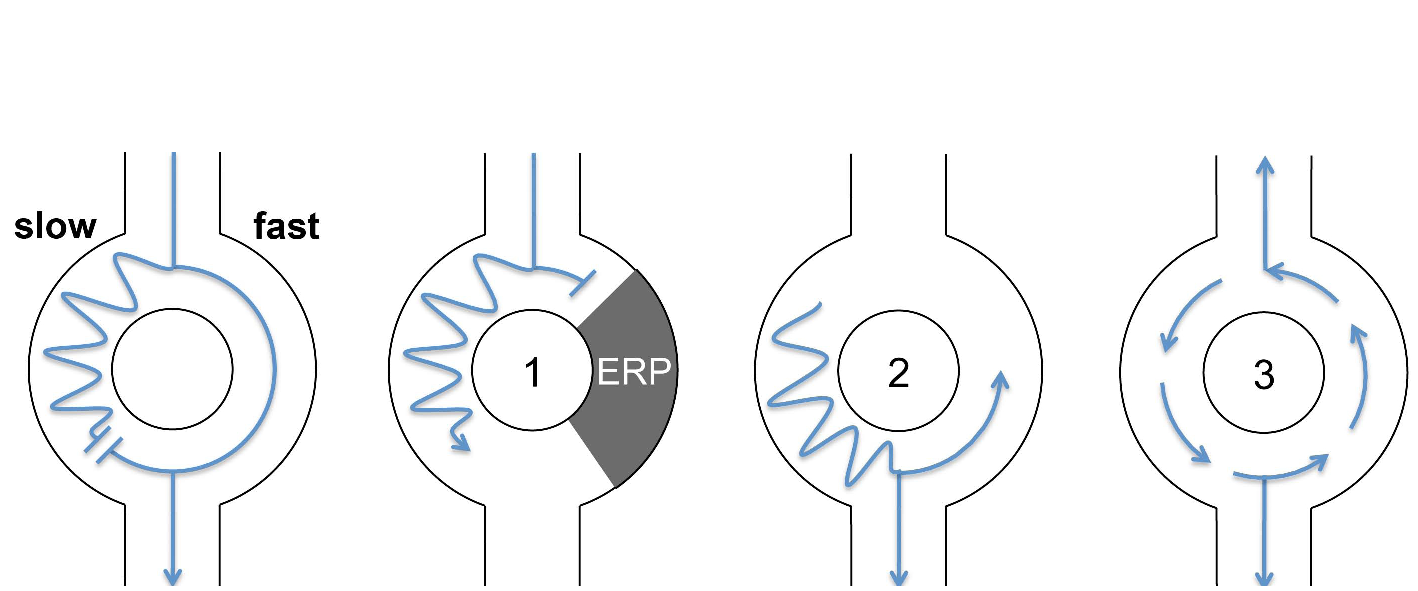
\includegraphics[width=0.6\textwidth]{figs/reentry.pdf}
%%\vspace{-5pt}
%\caption{\small Reentry Circuit}
%%\vspace{-15pt}
%\label{fig:reentry}
%\end{figure}
